\subsection{Exercise 15 from TAOCP ``7.1.3 Bitwise tricks and techniques''}

Page 53 from the fasc1a.ps, or: \url{http://www.cs.utsa.edu/~wagner/knuth/fasc1a.pdf}

\begin{figure}[H]
\label{fig:pipe_shuffled}
\centering
\frame{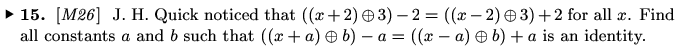
\includegraphics[scale=0.6]{SMT/TAOCP_7_1_3_exercise_15/page53.png}}
\caption{Page 53}
\end{figure}

Soltuion:

\begin{lstlisting}
from z3 import *

s=Solver()

a, b=BitVecs('a b', 4)
x, y=BitVecs('x y', 4)

s.add(ForAll(x, ForAll(y,  ((x+a)^b)-a == ((x-a)^b)+a  )))

# enumerate all possible solutions:
results=[]
while True:
    if s.check() == sat:
        m = s.model()
        print m

        results.append(m)
        block = []
        for d in m:
            c=d()
            block.append(c != m[d])
        s.add(Or(block))
    else:
        print "results total=", len(results)
        break
\end{lstlisting}

For 4-bit bitvectors:

\begin{lstlisting}

...

[b = 7, a = 0]
[b = 6, a = 8]
[b = 7, a = 8]
[b = 6, a = 12]
[b = 7, a = 12]
[b = 12, a = 0]
[b = 13, a = 0]
[b = 12, a = 8]
[b = 13, a = 8]
[b = 12, a = 4]
[b = 13, a = 4]
[b = 12, a = 12]
[b = 13, a = 12]
[b = 14, a = 0]
[b = 15, a = 0]
[b = 14, a = 4]
[b = 15, a = 4]
[b = 14, a = 8]
[b = 15, a = 8]
[b = 14, a = 12]
[b = 15, a = 12]
results total= 128
\end{lstlisting}

